\section{User Interface}
\label{sec:chapter_2_section_2}

Per definizione il software CAD è un acronimo inglese usato per indicare due concetti correlati, ma differenti:
\begin{itemize}
  \item Computer-Aided Drafting;
  \item Computer-Aided Design;
\end{itemize}
L'applicazione web che si è implementata, si presenta come un software CAD semplificato, dove la
user interface comprende:
\begin{itemize}
  \item 2D canvas (Figura~\ref{fig:view2D})
  \item 3D canvas (Figura~\ref{fig:viewer3D}).
\end{itemize}

L'area di lavoro (Figura~\ref{fig:interfaccia}) è suddivisa in aree ben specifiche,
le quali adempiono a funzionalità che verranno approfondite in dettaglio nei paragrafi successivi.\\

\begin{figure}[htbp] %  figure placement: here, top, bottom, or page
   \centering
   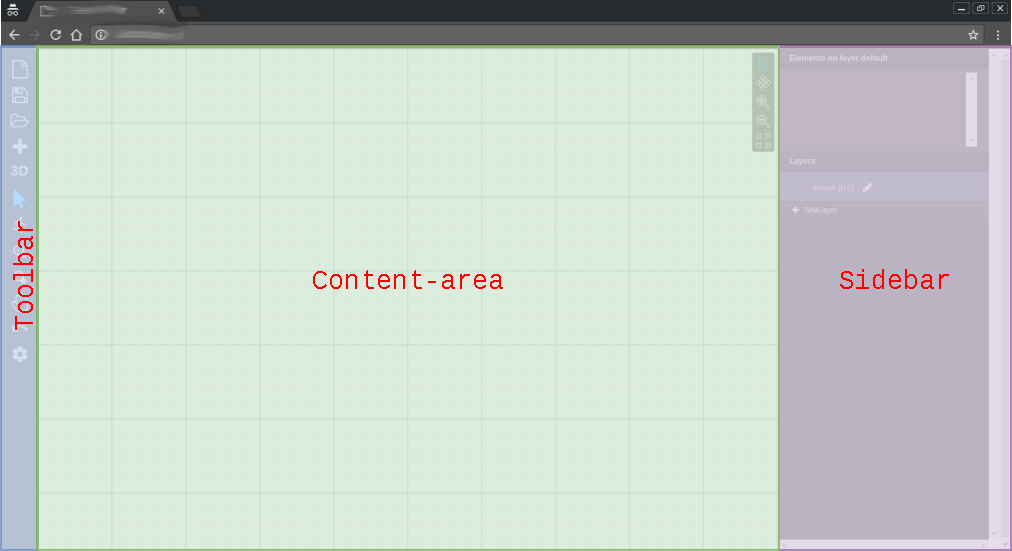
\includegraphics[width=1\linewidth]{images/mock-interfaccia}
   \caption{Schermata componenti interfaccia}
   \label{fig:interfaccia}
\end{figure}
\newpage
Dalla toolbar l'utente pu\`o accedere alle funzionalit\`a relative a: ciclo di vita del progetto (new, save, load);
view/interaction mode switching (2D, 3D); interaction mode changing (selecting, pan, zoom).
La content-area \`e un area nella quale l'utente pu\`o interagire con il modello attuale. Nella modalit\`a 2D
il modello \`e visualizzato come una proiezione 2D dall'alto e l'interazione consiste nell'inserimento, selezione e modifica
dell'elemento (in accordo con le specifiche interattive del prototipo). Nella modalità 3D un modello 3D pu\`o essere
inspezionato e navigato attraverso due modalità differenti: in prima persona usando il mouse e la tastiera ponendo la vista
ad altezza uomo, o dall'alto cambiando la posizione della telecamera con il solo mouse. Anche in modalità 3D è possibile
selezionare e posizionare gli oggetti.
La sidebar visualizza le propriet\`a dell'elemento correntemente selezionato. Nel pannello delle propriet\`a \`e possibile
vedere la descrizione dell'elemento, aggiungere/rimuovere metadata, e modificare qualsiasi propriet\`a.
Quest'ultima modalità di interazione consente al utente di associare annotazioni semantiche su ogni parte del modello.
\newpage

\subsection{Viewer 2D}
Il \emph{2D-viewer} invoca la funzione\emph{2Dgf} dei \emph{building elements} aggiunti al modello e genera in output il modello
renderizzato usando gli elementi SVG.
Per far fronte ai frequenti aggiornamenti provenienti dall'interazione con il disegno da parte dell'utente,
sfrutta la \emph{Virtual DOM}~\cite{vdom}, che permette di aggiornare solo la parte modificata evitando così
il completo rendering della scena. Per eseguire le operazioni di pan e zoom, tipicamente necessaria in questo
tipo di strumento, è stato sviluppato un componente ad-hoc
di React denominato \emph{ReactSVGPanZoom}\footnote{\url{https://github.com/chrvadala/react-svg-pan-zoom}}.\\

% The \emph{2D-viewer} invokes the \emph{2Dgf} of the building elements added to the model and renders its output using SVG
% elements. To cope with frequent updates coming from the user drawing interaction, it exploits the \emph{Virtual DOM}~\cite{vdom},
%  which permits to update only the modified part thus avoiding complete redrawing of the scene. To perform pan and zoom operations,
%   typically necessary in this kind of tool, we develop an ad-hoc React component named
  % \emph{ReactSVGPanZoom}\footnote{https://github.com/chrvadala/react-svg-pan-zoom}.

\begin{figure}[htbp] %  figure placement: here, top, bottom, or page
   \centering
   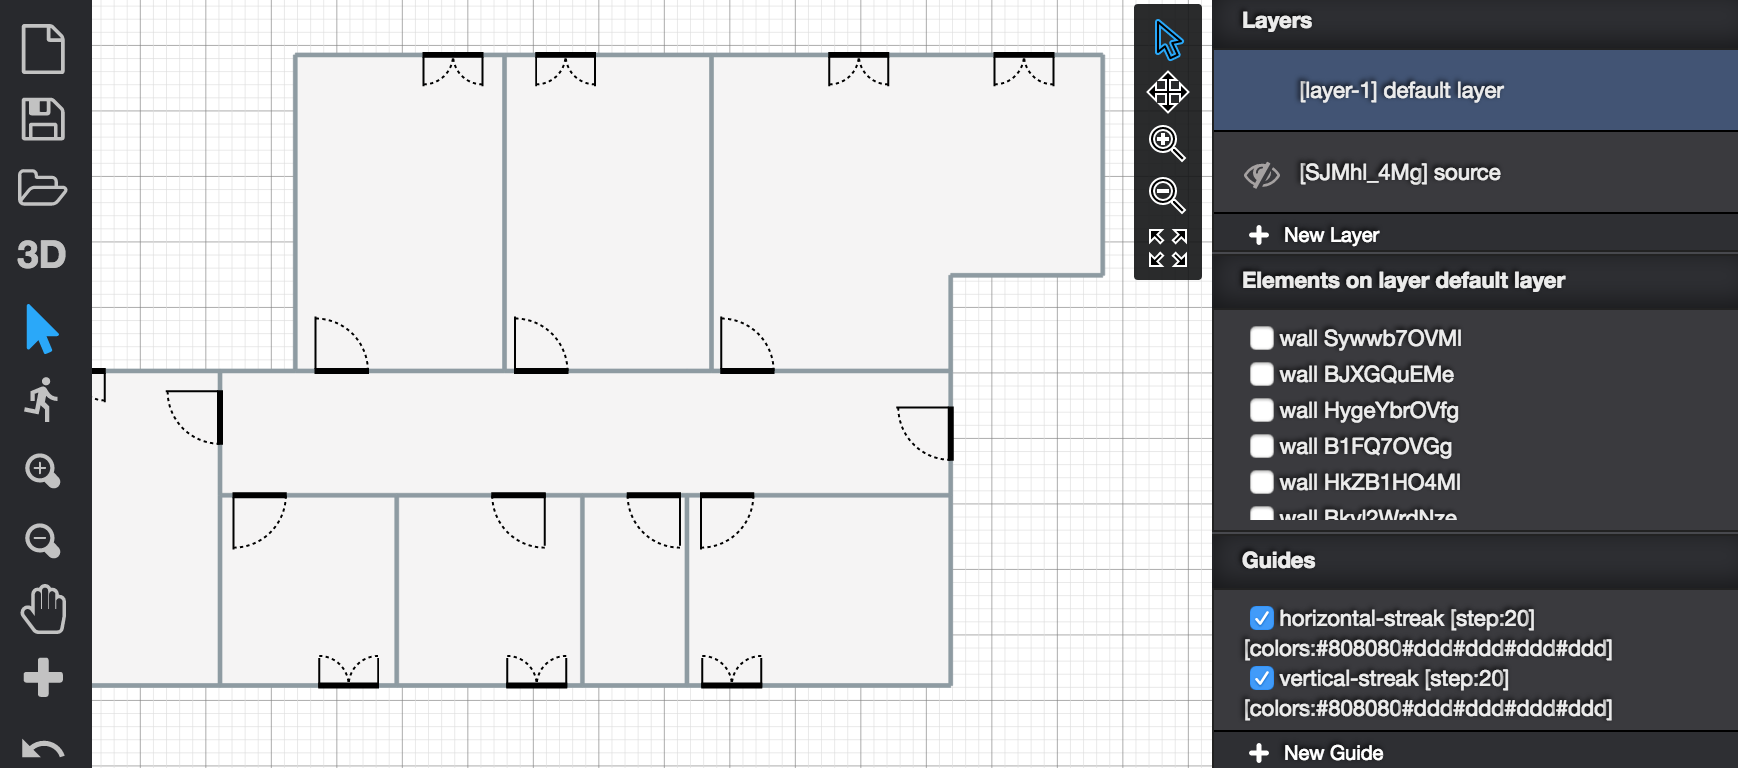
\includegraphics[width=1\linewidth]{images/2d}
   \caption{Schermata viewer 2D}
   \label{fig:view2D}
\end{figure}
\newpage


\subsection{Viewer 3D}
Il \emph{3D-viewer} invoca la funzione \emph{3Dgf} dei \emph{building elements} aggiunge al modello una vista 3D usando
le primitive WebGL\emph{Three.js}~\footnote{\url{https://threejs.org/}}. \`E stato implementato un \emph{diff} e \emph{patch} di
sistema, definite nel Jsonpatch~\cite{rfc6902}: gli oggetti Three.js sono associati con elementi costruttivi all'interno
dello stato dell'applicazione, in modo che ogni volta che l'utente attiva un'azione che si traduce in una modifica dello stato,
l'applicazione calcola la differenza tra il vecchio stato e quello nuovo e cambia solo l'oggetto interessato.
(spostare prima causa effetto delle azioni)
In particolare possiamo avere le seguenti \textit{operazioni}:
\begin{itemize}
  \item \emph{add};
  \item \emph{replace};
  \item \emph{remove};
\end{itemize}

% The \emph{3D-viewer} invokes the \emph{3Dgf} of the building elements added to the model and renders its output using WebGL
%  primitives via \emph{Three.js}~\footnote{https://threejs.org/}. It has been implemented a \emph{diff} and \emph{patch}
%  system, standardized in~\cite{rfc6902}: Three.js objects are associated with building elements inside the state, so every
%   time the user triggers an action that results in a state alteration, the application computes the difference between the
%    old state and the new one and changes only the affected object. In particular we can have the following \textit{operations}:
%     (i) \emph{add}, (ii) \emph{replace} and (iii) \emph{remove}.

\begin{figure}[htbp] %  figure placement: here, top, bottom, or page
   \centering
   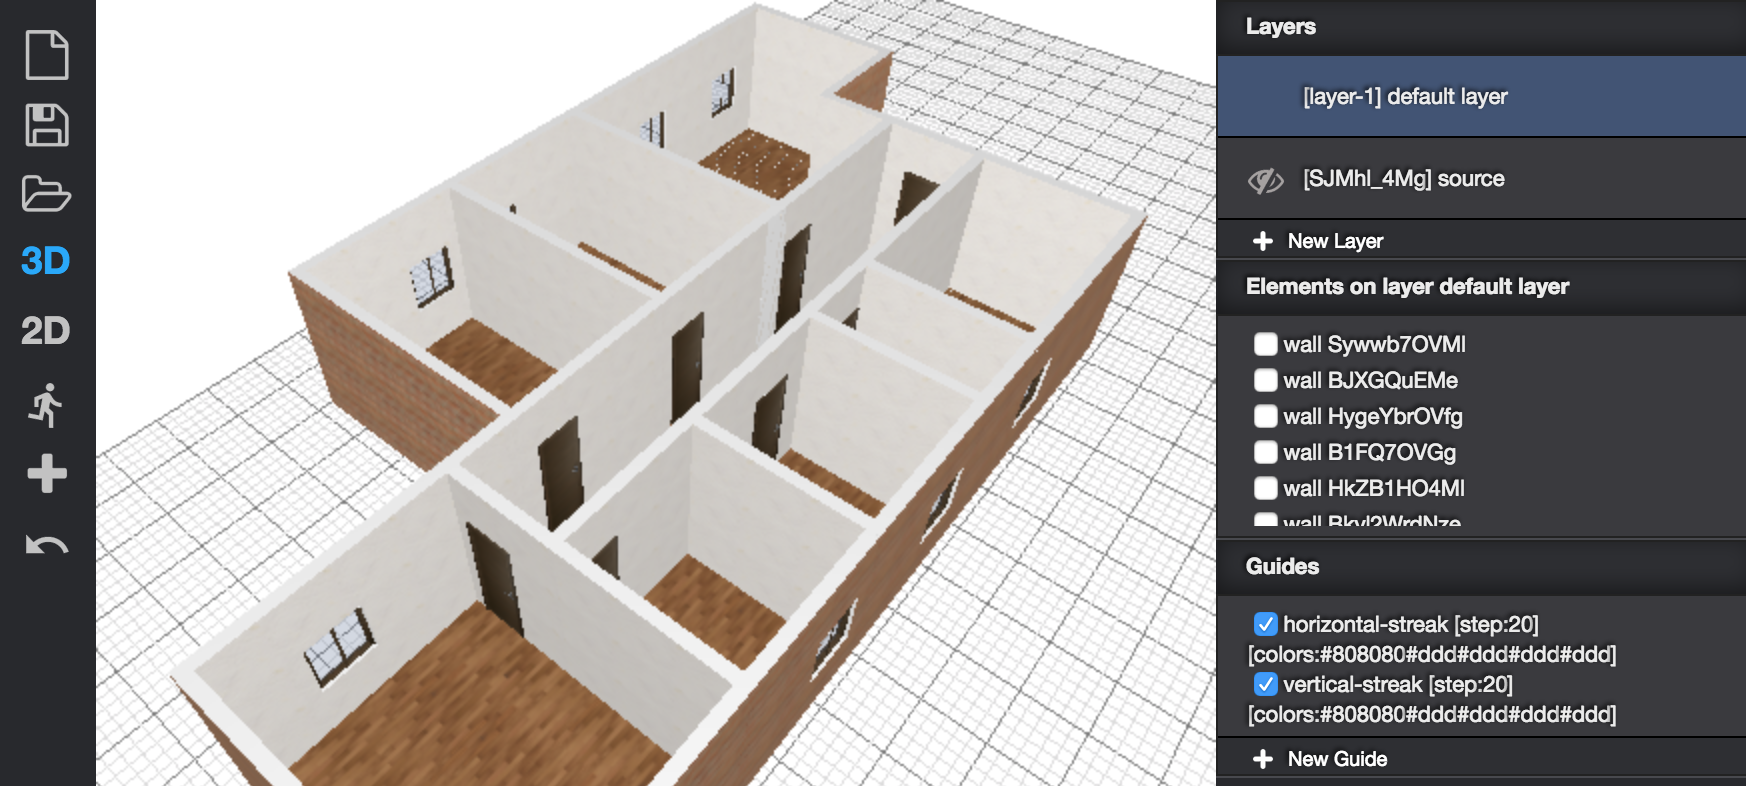
\includegraphics[width=1\linewidth]{images/3d}
   \caption{Schermata viewer 3D }
   \label{fig:viewer3D}
\end{figure}
\newpage

\subsection{Plugin Catalog}
\label{sec:chapter_2_section_2_sub_3}

\noindent
 Il plugin catalog \`e l'elemento centrale che fornisce all'utente un sistema con un ricco catalogo di plugin,
 in cui ogni elemento presente al suo interno \`e definito da un nome, una descrizione ed una
 immagine di anteprima del modello 3D (Figura~\ref{fig:figura1} (a)). Quando l'utente \`e al suo interno
 sceglie il plugin da inserire con un click dopo il quale si passa nella modalit\`a 2D-view, dove verrà posizionato
 all'interno della scena (Figura~\ref{fig:figura1} (b)).


\begin{figure}[htbp]
\begin{center}
\begin{tabular}{c @{\hspace{1em}} c}
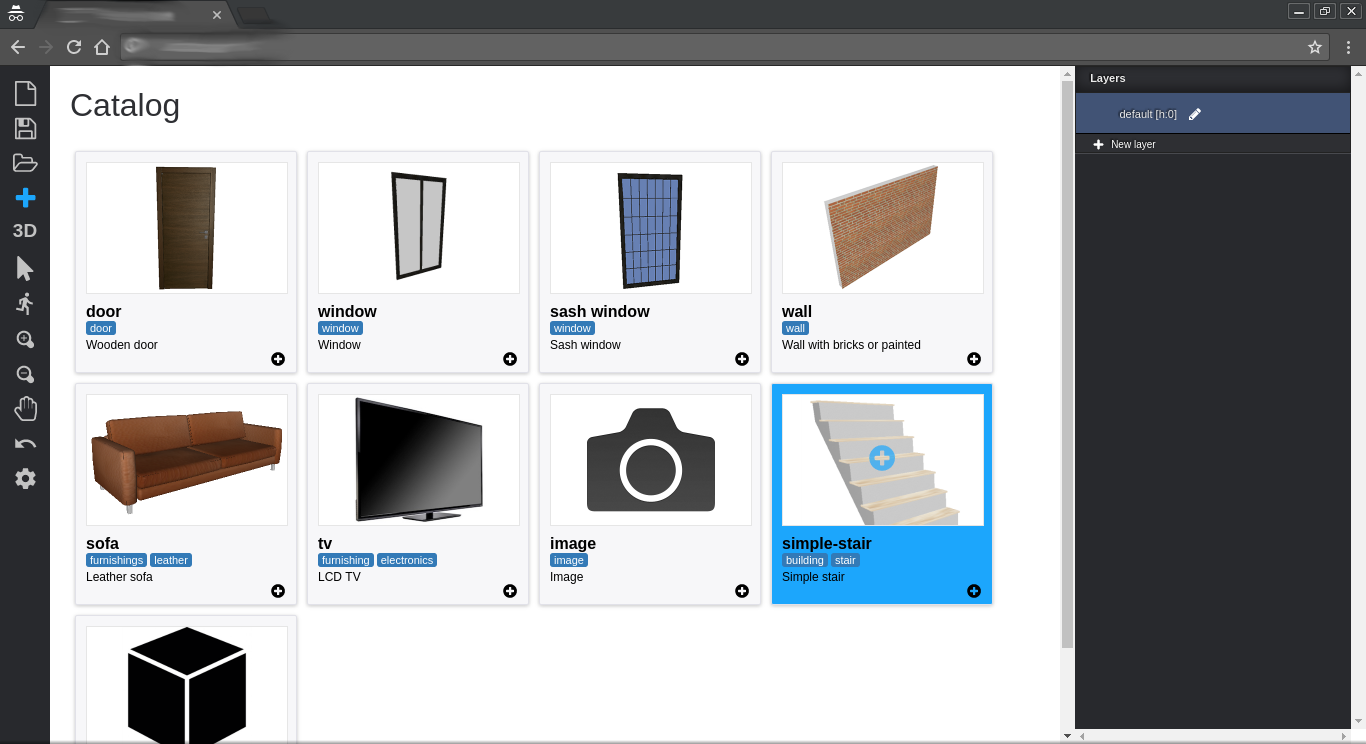
\includegraphics[width=9cm]{images/figcatalog} \\
  (a) \\
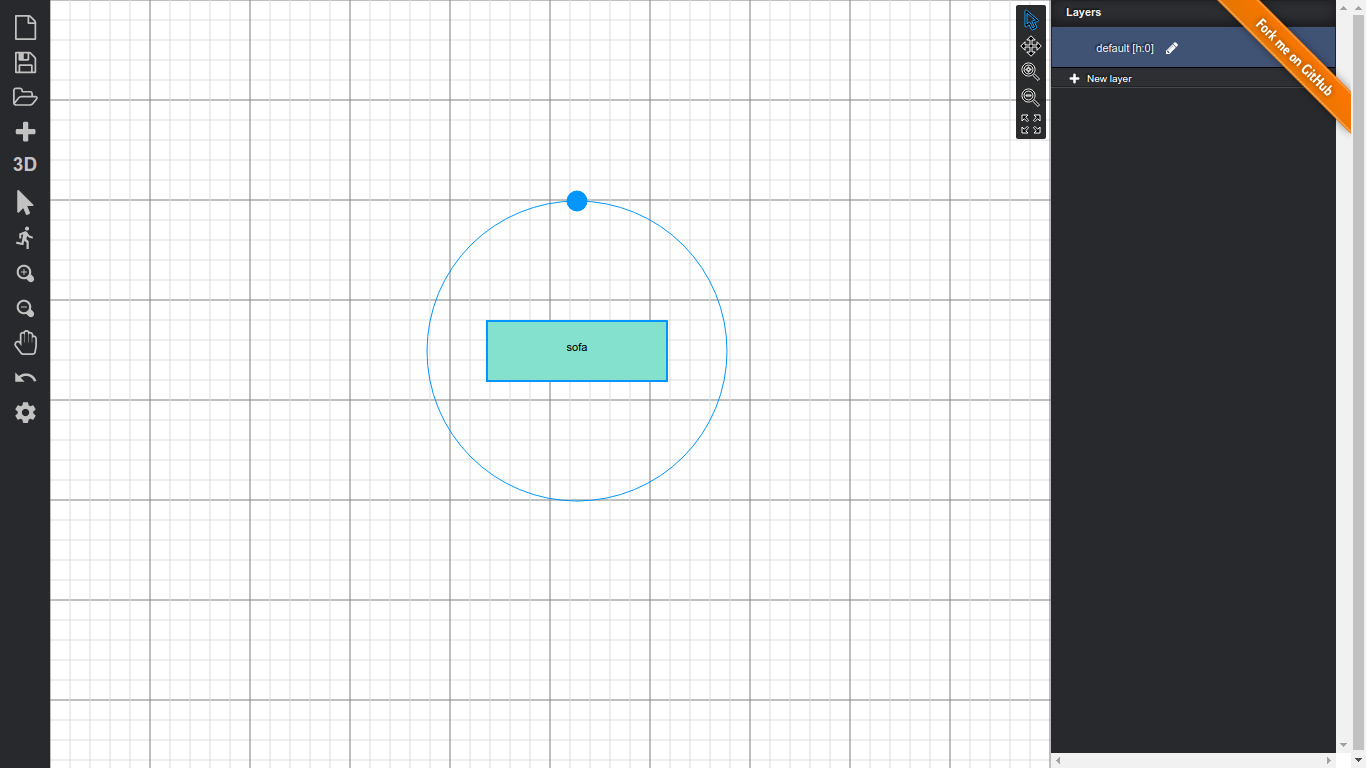
\includegraphics[width=9cm]{images/positioning} \\
  (b) \\
\end{tabular}
\end{center}
\caption{Dettaglio Plugin: (a) Vista dei plugin nel catalogo, (b) inserimento oggetto dopo la selezione nel catalogo}\label{fig:figura1}
\end{figure}
\newpage
